%%% LaTeX Template: Article/Thesis/etc. with colored headings and special fonts
%%%
%%% Source: http://www.howtotex.com/
%%% Feel free to distribute this template, but please keep to referral to http://www.howtotex.com/ here.
%%% February 2011
%%%
%%% Last updated September 2021 by CDM

%%%  Preamble
\documentclass[11pt,letterpaper]{article}
\usepackage[margin=1.0in]{geometry}
\usepackage[T1]{fontenc}
\usepackage[bitstream-charter]{mathdesign}
\usepackage[latin1]{inputenc}					
\usepackage{amsmath}						
\usepackage{xcolor}
\usepackage{cite}
\usepackage{hyphenat}
\usepackage{graphicx}
\usepackage{float}
\usepackage{subfigure}
\usepackage{sectsty}
\usepackage[compact]{titlesec} 
\usepackage[tablegrid]{vhistory}
\allsectionsfont{\color{accentcolor}\scshape\selectfont}
\usepackage{indentfirst}

%%% Definitions
\definecolor{accentcolor}{rgb}{0.0,0.0,0.5} 
\newcommand{\teamname}{NursingBros}
\newcommand{\productname}{SmartInventory \textsuperscript{TM}}
\newcommand{\coursename}{CSE 4316: Senior Design I}
\newcommand{\semester}{Summer 2022}
\newcommand{\docname}{Project Charter}
\newcommand{\department}{Department of Computer Science \& Engineering}
\newcommand{\university}{The University of Texas at Arlington}
\newcommand{\authors}{Nguyen Le \\ Alexander Martinez \\ Kennedy Mosoti \\ Bradley Norman}

%%% Headers and footers
\usepackage{fancyhdr}
	\pagestyle{fancy}						% Enabling the custom headers/footers
\usepackage{lastpage}	
	% Header (empty)
	\lhead{}
	\chead{}
	\rhead{}
	% Footer
	\lfoot{\footnotesize \teamname \ - \semester}
	\cfoot{}
	\rfoot{\footnotesize page \thepage\ of \pageref{LastPage}}	% "Page 1 of 2"
	\renewcommand{\headrulewidth}{0.0pt}
	\renewcommand{\footrulewidth}{0.4pt}

%%% Change the abstract environment
\usepackage[runin]{abstract}			% runin option for a run-in title
%\setlength\absleftindent{30pt}			% left margin
%\setlength\absrightindent{30pt}		% right margin
\abslabeldelim{\quad}	
\setlength{\abstitleskip}{-10pt}
\renewcommand{\abstractname}{}
\renewcommand{\abstracttextfont}{\color{accentcolor} \small \slshape}	% slanted text

%%% Start of the document
\begin{document}

%%% Cover sheet
{\centering \huge \color{accentcolor} \sc \textbf{\department \\ \university} \par}
\vspace{1 in}
{\centering \huge \color{accentcolor} \sc \textbf{\docname \\ \coursename \\ \semester} \par}
\vspace{0.5 in}
\begin{figure}[h!]
	\centering
   	
\includegraphics[width=0.60\textwidth]{images/smart_inventory_logo.jpg}
\end{figure}
\vspace{0.5 in}
{\centering \huge \color{accentcolor} \sc \textbf{\teamname \\ \productname} \par}
\vspace{0.5 in}
{\centering \large \sc \textbf{\authors} \par}
\newpage


%\vspace{1 in}
%\centerline{January 13th, 2012}
%\newpage

%%% Revision History
\begin{versionhistory}
  	\vhEntry{0.1}{06.22.2022}{AM}{document creation}
  	\vhEntry{0.2}{06.28.2022}{NI|AM|KM|BN}{project charter draft 1}
\end{versionhistory}
\newpage

%%% Table of contents
\tableofcontents
\newpage

%%% List of figures and tables (optional)
\listoffigures
\listoftables
\newpage
\setcounter{table}{0}

%%% Executive summary sections
\section{Problem Statement}
% The problem statement defines the "Why" of the project. This is the higher purpose, or the reason for the project's existence. This section should avoid mentioning implementation details, and focus more on what the current problem is and what would be gained if the problem were to be solved. In short, the is the reason that you are going to be working on something, not the method(s) that you will be employing.

Inventory control has always played a vital role in any industry, especially in the healthcare industry - where the patient's health and life can depend on a tool or a piece of equipment. Inventory management is lengthy and challenging since it is prone to human error. A smart inventory management application will be a great solution to solve all these problems.
\section{Methodology}
% This is the "What" of the project and it states what will be done to address the problem statement. This section should focus mostly on what your solution is going to be and what it is going to do (i.e., we are going to build an app, robot, device, etc. to perform some task which mitigates the problem). If someone were to ask you \textit{"What are you doing for your senior design project?"}, this is section is basically what you would tell them.

We are going to develop an inventory management application with the right approach and methodology to mitigate some of the biggest problems in inventory management. Using the app, users can fill out and submit loan equipment application forms online. This replaces the old process of having to meet the inventory administrator in person and fill out a paper form. We believe this will speed up the loaning equipment process, and save time for both the loaner and the loanee. Utilizing a cloud database, having the data automatically sync to the cloud instead of saving the file locally and manually backing up the data - will help the inventory administrator not to worry about losing the data in their machine. And last but not least, a future-proof, highly customizable inventory database system will help the administrator to add/remove any piece of equipment on demand.
\section{Value Proposition}
%The Value Proposition explains how the sponsors will benefit from your work, and why they should invest funding, time, and expertise in supporting your team. Here, you are essentially making a case for the project. There are many ways in which value can be returned to your stakeholders (industrial sponsors, instructors, the university, etc.), list any that may help you convince them to "buy in".

%We help (X) do (Y) by doing (Z).

The SmartInventory application will benefit our customer by providing them with the ability to easily and readily manage their inventory. By reducing the amount of time our customer spends having to manually keep track and delegate their inventory assets, SmartInventory will allow our customer to conduct business in a more efficient manner. Additionally, SmartInventory will allow our customer to save as the application is offered at a rate far cheaper than that of current competitors in the market.
\section{Development Milestones}
This list of core project milestones should include all major documents, demonstration of major project features, and associated deadlines. Any date that has not yet been officially scheduled at the time of preparing this document may be listed by month.
\\
\\
Provide a list of milestones and completion dates in the following format:
\begin{itemize}
  \item Project Charter first draft - June 29\textsuperscript{th}, 2022
  \item System Requirements Specification - July 13\textsuperscript{th}, 2022
  \item Architectural Design Specification - July 27\textsuperscript{th}, 2022
  \item Demonstration of Database - August 2022
 % \item Detailed Design Specification - Month Year
  \item Demonstration of Basic Database Interface  - September 2022
  \item Demonstration of Database API - September 2022
 % \item CoE Innovation Day poster presentation - Month Year
  \item Demonstration of Item Checkout Features - October 2022
  \item Demonstration of Reports system  - November 2022
  \item Demonstration of Prototype used for move - November 2022
  \item Final Project Demonstration - December 2022
\end{itemize}
\newpage

%%% Remaining project charter sections
\section{Background}
%An in-depth explanation of the problem, including the "business case". What is wrong with the status-quo or what opportunity exists that justifies undertaking this project (expanding upon the problem statement)? If you have a clear customer or sponsor, why do they want you to work on this? What is the existing relationship, if any, between the development team and the customer? This section should occupy 1/2 - 1 full page.

The current problem with inventory system in place now is that it takes tremendous effort by our customer to keep track of all items in the system. The current system consists of an excel spreadsheet that is used to track each individual asset in the nursing department's inventory which amounts to more than 150 assets (not including non-assets) located in two different buildings on UTA's campus. Requests for use of inventory items are handled using physical forms which document the purpose and time on which an asset is checked out for use. Items checked out for an extended period of time would require a constant reminder that they are still in use by, in our customer's case, hanging the document on a board. Accessing and editing the excel spreadsheet is all conducted from the Simulation Inventory Specialist's computer. The excel sheet is solely managed by one person in the department, The Simulation Inventory Specialist, in which they are responsible for processing requests, repairs, and the retirement of the equipment on a day-to-day basis. 

Our customer requests the development of the SmartInventory application to help reduce the load of work on the individual specialist working on the current inventory system. There currently isn't a development team on hand working on this specific solution so this will be a fresh approach to develop this application. One of the aims of this assignment is to develop a relationship with our customer in order to deliver a solution that satisfies their needs and also provide a inventory application that minimizes the occurrence of human error. 
\section{Related Work}
%Discuss the state-of-the-art with respect to your product. What solutions currently exist, and in what form (academic research, enthusiast prototype, commercially available, etc.)? Include references and citations as necessary using the \textit{cite} command, like this \cite{Rubin2012}. If there are existing solutions, why won't they work for your customer (too expensive, not fast enough, not reliable enough, etc.). This section should occupy 1/2 - 1 full page, and should include at least 5 references to related work. All references should be added to the \textit{.bib} file, fully documented in IEEE format, and should appear in the \textit{references} section at the end of this document (the IEEE citation style will automatically be applied if your reference is properly added to the \textit{.bib} file).

%ProTip: Consider using a citation manager such as Mendeley, Zotero, or EndNote to generate your \textit{.bib} file and maintain documentation references throughout the life cycle of the project.

In researching other options it appears that none of them quite match what the College of Nursing is needing. One of the more popular options that is offered by Oracle is NetSuite. This system appears to be more of an total workplace management system with more features than needed as it is more suited for a warehouse setting \cite{costello_2021}. Another related product that is being used currently was Excel. Currently the Simulation Inventory Specialist is manually tracking all of the items with a few pages. The problem with this solution is that it is very involved and time consuming. Fishbowl is another resource that could be used by the nursing department. In researching this product negative reviews where found about working with the company. This along with it's large price tag make it a poor candidate \cite{g2}. An additional Software that is close to NetSuite is Sage Intacct. Sage appears to be more of a financially focused software rather then one that keeps tabs on locations of inventory items \cite{capterra}. A software that seems to be more closely related to the needs of the nursing department is Zoho Inventory. This software is offered with a free version, so the price point matches the budget of the nursing department. But once again the functionality of this program seems to be for the selling of products rather than the tracking of where they go \cite{inventory}. Further research yielded an article by nerdwallet that provided a large list of different inventory management systems \cite{wood_2021}. All seemed to support a business that are selling their products rather then keeping tabs on their whereabouts.

From our research it appears that the niche needs of the nursing department have no Related Software that fits for them. The ability to schedule service for some assets  This shows us that for multiple reasons the nursing department has chosen to forgo other inventory management systems. 
\section{System Overview}
%Explain, at a high level, how you will implement a solution to the problem. Include a diagram of major components to the system (not a full architectural design, but a high level overview of the major system components and how a user or external system might interface). Avoid specific implementation details (operating system, programming languages, etc.). This section should occupy at least 1 full page.

The application will be a full stack application where the user interacts with an inventory interface that allows them to view and request items from the equipment inventory. The Application will allow for the admin, in this case the Simulation Inventory Specialist, to customize there own categories as needed as well as add items. These items will have a unique identifier or bar code as well as the location of said item. Some items that are worth upwards of \$5,000.00 are classified as assets and are tracked using UTA's own tracking system. Our database will conform to these codes and allow for customization of bar codes at entry. Possibly the most important part of this inventory system will be an interface that allows a Actor level user to edit the database. This is because the admin will have zero coding experience.

The flow of command will begin with an instructor requesting an item to be checked out. This will then be approved by the admin and marked in the GUI. The database will be updated to the changes. After the item is finished it will either be returned to the storage area or removed from the database depending on the item's classification.

Another key component to the inventory system will be a timer attached to all checked out items.  This is per the nursing departments rule of a 72 hour check out limit for assets and non-assets. The extension of this timer will also have to be reset about approval from Simulation Inventory Specialist. Request to extend might be able to take place in application. 

On top of the check out system we will need a system to retain the locations of all items as well as the instructor that has them checked out if applicable. This will include the room numbers and section of room if applicable. The minutiae of this will have to be further fleshed out as they are currently moving facilities. Also in the item description there will  need to be a section that shows purchase history. Related to this there will also need to be an option to set up a maintenance schedule for some of the items that require it.

Consumables will be another item that will have to be recorded. They will be a special category that will build up as items are ordered so adding to a number of current items in the system will be needed. After Items are checked out they will be decremented from the count. This should be automated to allow for ease of use on the part of the administrator.

The final known requirement will be to create mass checkouts or 'labs' that will allow for the admin to add multiple items in one cart and apply the same status of location and owner to all of them. Also in this will the adding the consumables that are automatically taken out of the running count.

\begin{figure}[h!]
	\centering
   	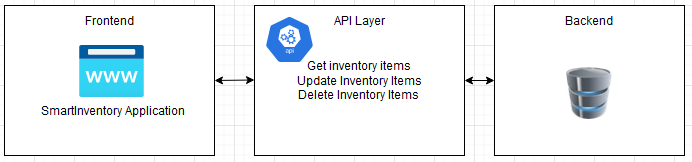
\includegraphics[width=0.60\textwidth]{images/Component_Diagram.png}
   	\centering
   	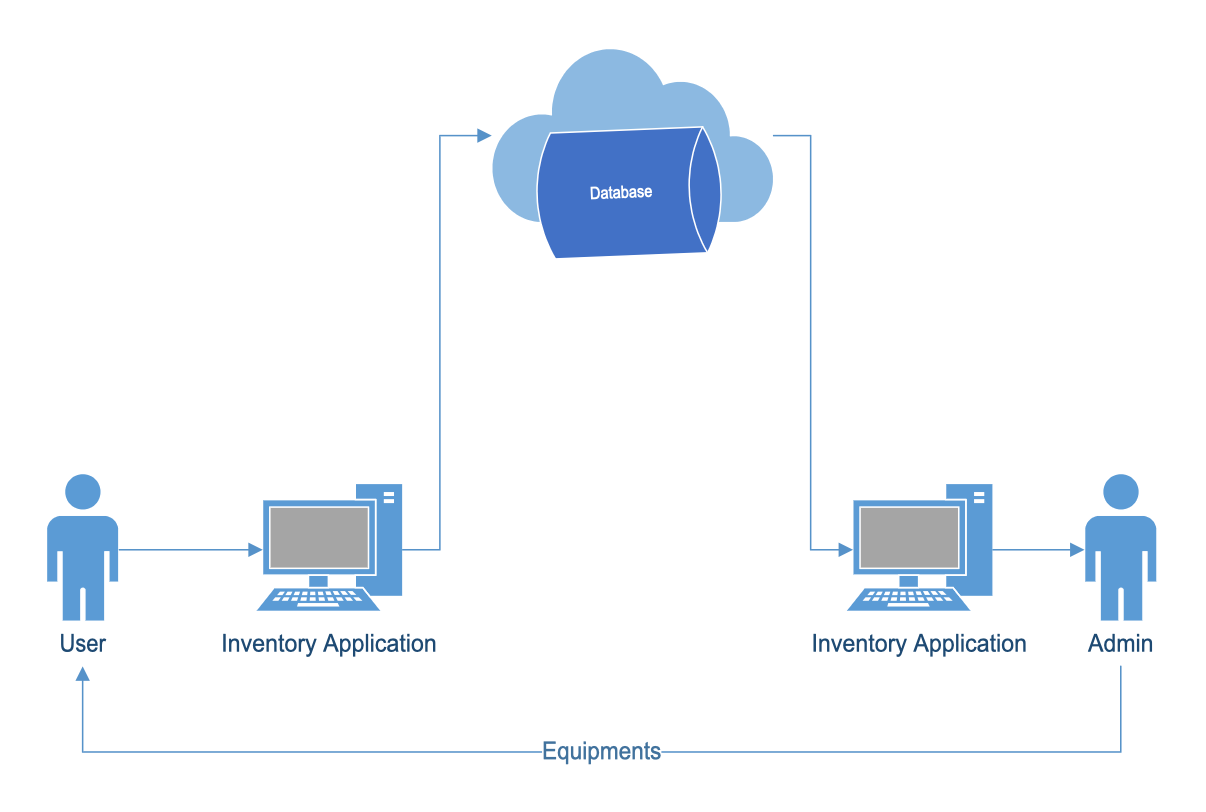
\includegraphics[width=0.60\textwidth]{images/User_Data_Flow.png}
\end{figure}


\section{Roles \& Responsibilities}
%Who are the stakeholders of the project? Who will be the point of contact from the sponsor or customer side? Who are the team members, and what will be their areas of responsibility? Will your team maintain the product owner and scrum master for the whole project, or will that role change periodically? This section should occupy 1/2 - 1 full page.
Aside from the team members of the SmartInventory App being shareholders, the Simulation Inventory Specialist for the Nursing Department, Jacquelyn Donaldson, is also a shareholder. Nguyen Le, Alexander Martinez, Kennedy Mosoti, and Bradley Norman compose of the team members, which is a combination of half software engineers and other half computer scientists.

Bradley Norman will be point of contact for our sponsor and customer, Jacquelyn Donaldson, using Outlook UTA email to communicate  and schedule meetings before and after sprints or whenever each party deems it necessary. The title scrum master will be change periodically to allow each member the opportunity to experience leadership.

Since the project will be divided in three areas: Front-end, Application Programming Interface (API), and Back-end. We will attempt to divide the work evenly as much as possible, by having Kennedy and Bradley work on the Front-end while simultaneously Alexander and Nguyen working on the Back-end. Then converging collaboratively on the API. The Front-end is what the SmartInventory Application which the users see's, all the different graphic user interface options. The API is how the Front-end and Back-end interact, sending or receiving data. The Back-end is where all the data is stored for the assets and non-assets. As a whole, we all have a responsibility to help one another if they are struggling. For example, the pair team members are struggling on a area, then the other pair of team members needs to drop what they are doing to help or if one of the pair of team members one is struggling, then the other half of the pair needs to assist them. If this project is going to succeed and finish on time, then ensuring every member of the team is on board. Also, guide one another with the course submission's making sure everyone completes the course and succeeds. Finally, we all have the responsibility to communicate with one another, to the team as a whole effectively, and to Jacquelyn Donaldson, so there are no ambiguity to the development process throughout these two semesters of the course.
\section{Cost Proposal}
%This section contains the approximate budget for the project, where that money will come from, and any other support. This text should be replaced with a discussion and justification of major expenses, but not the actual monetary amounts (that will go in the preliminary budget section below). 


\subsection{Preliminary Budget}
%Include a high level budget table for components, fabrication, software licensees, development hardware, etc. This should be in a tabular format broken up into appropriate line items. 


\begin{table}[h]
\centering
\resizebox{0.8\textwidth}{!}{
\begin{tabular}{|l|l|}
\hline
 \textbf{Item} & \textbf{Cost} \\ \hline
 Cloud Computing Services- AWS   & \$50 per month or \$300 \\ \hline
 Bar code Scanner Printer   & \$70 \\ \hline
 React Native   & Free \\ \hline
\end{tabular}}
\caption{Overview of preliminary budget} 
\end{table}

\subsection{Current \& Pending Support}
%What are all of the funding sources for the project, and are there any potential funding sources that haven't been secured yet? List all funding sources (including the default funding amount provided by the CSE department) and their dollar amounts.


\begin{table}[h]
\centering
\resizebox{0.8\textwidth}{!}{
\begin{tabular}{|l|l|}
\hline
 \textbf{Source} & \textbf{Amount} \\ \hline
 Department of Computer Science and Engineering   & \$800 \\ \hline
\end{tabular}}
\caption{Overview of funding sources} 
\end{table}
\section{Facilities \& Equipment}
%What lab space, testing grounds, makerspaces, etc. will you need to complete the project? Will you require any specific equipment, and if so, where will you get it (borrow, lease, purchase, outsource, already present in the lab, etc.). This section should occupy 1/2 page.
The team will use the senior design labs in ERB 208 to have a dedicated workspace to be able to work on the project distraction free, and store equipment like a bar code scanner and bar code scanner printer. Access to the Smart Hospitals Inventory in the Smart Hospital building and in the University Hall building to mark down where individual assets and non-assets are located (room, storage container type, row location, etc.), to be able to insert that data to the cloud-base database for inventory management later on. Later on access to the currently almost constructed building on campus where the assets are going to be stored for the same reason stated previously. Equipment that's not tangible that we need is a cloud-base database AWS from Amazon. Also an account with React Native. We don't need any other specific equipment because this is a software intense project. 
\section{Assumptions}
%The following list contains critical assumptions related to the implementation and testing of the project.

\begin{itemize}
  \item Testing will be done with the shareholder.
  \item Working prototype will be able to assist in move to new building.
  \item After deployment system will be able to be entirely managed by nursing department.
  \item Database will be backed up in case of catastrophic failure.
  \item If time permits, branch out to mobile app.
\end{itemize}
\section{Constraints}
%Constraints are limitations imposed on the project, such as the limitation of cost, schedule, or resources, and you have to work within the boundaries restricted by these constraints. All projects have constraints, which are defined and identified at the beginning of the project.

%Constraints are outside of your control. They are imposed upon you by your client, organization, government regulations, availability of resources, etc. Occasionally, identified constraints turn out to be false. This is often beneficial to the development team, since it removes items that could potentially affect progress.

%This section should contain a list of at least 5 of the most critical constraints related to your project. For example:

%The following list contains key constraints related to the implementation and testing of the project.

\begin{itemize}
  \item Final prototype demonstration must be completed by December 8\textsuperscript{th}, 2022
  %\item The customer will provide no more than two maintenance personnel to assist in on-site installation
  %\item Customer installation site will only be accessible by development team during normal business hours
  \item Customer should be able to reliable use the project inventory system in place of the current implementation
  \item Total development costs must not exceed \$800
  \item Inventory database will be hosted in a cloud environment
  \item All data obtained from customer site must be reviewed and approved for release by the Information Security Office prior to being copied to any internet connected storage medium
  \item Nursing department moving assets and non-assets to a newly constructed building in the fall 2022
\end{itemize}

\section{Risks}
%This section should contain a list of at least 5 of the most critical risks related to your project. Additionally, the probability of occurrence, size of loss, and risk exposure should be listed. For size of loss, express units as the number of days by which the project schedule would be delayed. For risk exposure, multiply the size of loss by the probability of occurrence to obtain the exposure in days. For example:

%The following high-level risk census contains identified project risks with the highest exposure. Mitigation strategies will be discussed in future planning sessions.

\begin{table}[h]
\resizebox{\textwidth}{!}{
\begin{tabular}{|l|l|l|l|}
\hline
 \textbf{Risk description} & \textbf{Probability} & \textbf{Loss (days)} & \textbf{Exposure (days)} \\ \hline
 Human Errors (Bugs)   & 0.50 & 20 & 10 \\ \hline
 Inadequate Developer Availability   & 0.20 & 14 & 2.8 \\ \hline
 Implementing End-user Test Results  & 0.30 & 9 & 2.7 \\ \hline
 Insufficient QA Testing   & 0.10 & 10 & 1.0 \\ \hline
 Loss of Internet Connection & 0.20 & 1 & 0.2 \\ \hline
\end{tabular}}
\caption{Overview of highest exposure project risks} 
\end{table}
\section{Documentation \& Reporting}
%%% In this section, you will describe all of the various artifacts that you will generate and maintain during the project life cycle. Describe the purpose of each item below, how the content will be generated, where it will be stored, how often it will be updated, etc. Replace the default text for each section with your own description. Reword this paragraph as appropriate.

\subsection{Major Documentation Deliverables}

\subsubsection{Project Charter}
%%Describe how this document will be maintained and updated (how often, under what circumstances, etc.). When will the initial version be delivered? When will the final version be delivered?
This document will be maintained and updated on a sprint-by-sprint basis after group discussion in the cases that new risks emerge, new items need to be added to the budget, etc.. The initial version of this document will be delivered on June 29, 2022, while the final version of this document will be delivered August 12, 2022.

\subsubsection{System Requirements Specification}
%Describe how this document will be maintained and updated (how often, under what circumstances, etc.). When will the initial version be delivered? When will the final version be delivered?
This document will be maintained through each update we have on our product and updated as necessary when the need for higher system requirements is needed. The initial version of this document will be delivered on July 13, 2022, while the final version of this document will be delivered August 12, 2022.

\subsubsection{Architectural Design Specification}
%Describe how this document will be maintained and updated (how often, under what circumstances, etc.). When will the initial version be delivered? When will the final version be delivered?
This document will be maintained and updated as needed when making changes to the framework of our initial design mock-up. The initial version of this document will be delivered on July 27, 2021, while the final version of this document will be delivered August 12, 2022.

\subsubsection{Detailed Design Specification}
%Describe how this document will be maintained and updated (how often, under what circumstances, etc.). When will the initial version be delivered? When will the final version be delivered?
The document will be maintained and updated any time we need to make a change to the structure of our code or to the system specifications to the hardware needed. The initial version of this document will be delivered on  , while the final version of this document will be delivered August 12, 2022.

\subsection{Recurring Sprint Items}

\subsubsection{Product Backlog}
%How will items be added to the product backlog from the SRS? How will these items be prioritized? Who makes the decision (product owner, group vote, etc.)? What software will be used to maintain and share the product backlog with team members and stakeholders?
When adding items to our product backlog we will hold a team meeting either in person or virtually through Discord to discuss whether it is added and the priority it will receive relative to the other items on the backlog currently. We will simply be using a combination of Outlook email and Discord group messaging to claim tasks and log hours for those tasks.

\subsubsection{Sprint Planning}
%How will each sprint plan be planned? How many sprints will there be (you need to look at the schedules for this course and previous Senior Design II courses during the appropriate semesters to figure this out).
Each sprint will be planned out around what immediate tasks need to get done regarding documentation and what needs to be done to progress in the development of our actual product. There will be 8 sprints total split equally between SD I and SD II.

\subsubsection{Sprint Goal}
%Who decides the sprint goal? How will you involve your customer in this process?
All members coming to consensus will be the primary decision maker on each sprint goal after group discussion and input. We will meet with the customer each sprint to ensure the sprint goal has met their requirements.

\subsubsection{Sprint Backlog}
%Who decides which product backlog items make their way into the sprint backlog? How will the backlog be maintained (collaboration software, a "scrum board", etc.)?
Each sprint we will come together as a group and decide which product backlog items will need to be added into the sprint backlog to be worked on. The sprint backlog will be maintained on through group messaging on Discord to determine what items are currently being worked on and by whom.

\subsubsection{Task Breakdown}
%How will individual tasks be assigned from the sprint backlog? Will it be up to each team member to voluntarily claim a task, or will it come from the product owner? How will time spent on tasks be documented?
Individual tasks from the sprint backlog will initially be taken on a voluntary basis and if there are still important items that must be done it will then be either done as a group or assigned to individuals.

\subsubsection{Sprint Burn Down Charts}
Which ever team member is first in generating burn down charts for each sprint. This person will be able to access the total amount of effort expended by each team member through logging hours on a shared discord server.

\begin{figure}[h!]
    \centering
    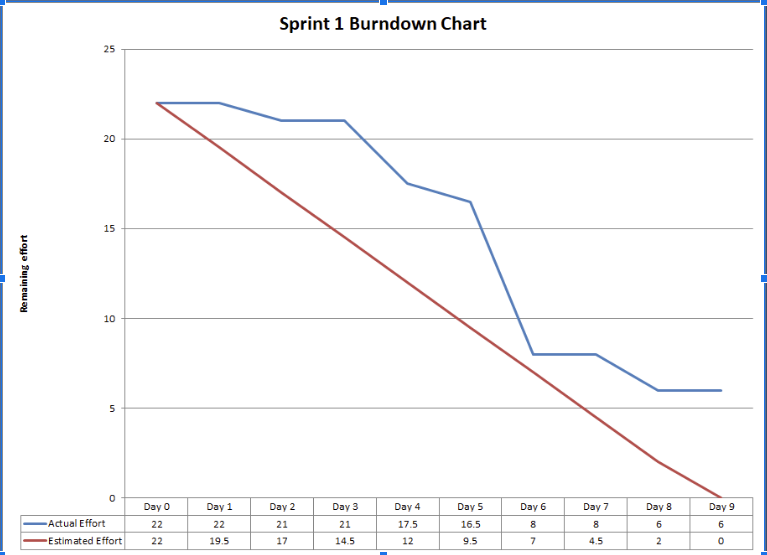
\includegraphics[width=0.5\textwidth]{images/sprint1_burndown.png}
    \caption{Example sprint burn down chart}
\end{figure}

\subsubsection{Sprint Retrospective}
%How will the sprint retrospective be handled as a team? When will this discussion happen after each sprint? What will be documented as a group and as individuals, and when will it be due?
The sprint retrospective be handled as a regular team meeting and will be held around the end of the current sprint. Meeting details will be documented within engineering notebooks per individual as normal.

\subsubsection{Individual Status Reports}
%What sort of status will be reported by each individual member, and how often will it be reported? What key items will be contained in the report?
The general status to be reported by each individual member will be the sprint backlog along with their time expenditure spent on each task that was worked on every 1.5 weeks/sprint duration. The major key items to be reported will be an individual retrospective and a peer review to conclude each sprint.

\subsubsection{Engineering Notebooks}
%How often will the engineering notebook be updated, at a minimum, by each team member? What is the minimum amount of pages that will be completed for each interval, and how long will that interval be? How will the team keep each member accountable? Who will sign of as a "witness" for each ENB page?
The engineering notebook will be updated once a week minimum, with a minimum of 1 page during the 1.5-week sprint interval. We will keep each other accountable through meetings to share new findings, updates, research, etc. weekly.

\subsection{Closeout Materials}
%The following materials, in addition to major documentation deliverables, will be provided to the customer upon project closeout. Remove this paragraph from your draft, but leave the heading.

\subsubsection{System Prototype}
%What will be included in the final system prototype? How and when will this be demonstrated? Will there be a Prototype Acceptance Test (PAT) with your customer? Will anything be demonstrated off-site? If so, will there be a Field Acceptance Test (FAT)?
The Final prototype will include a working database along with a barcode system that tracks the items. This system will also have the ability to check out items and track their whereabouts based in. Testing will be done in conjunction with the Simulation Inventory Specialist to ensure that all requirements are met.

\subsubsection{Project Poster}
%What will be included on the poster, what will be the final dimensions, and when will it be delivered?
Poster will Include screenshots of the GUI as well as information related to the Nursing Simulation Classes to better inform others of what this Application will do. Poster will be on a regular 36" by 48" poster board.

\subsubsection{Web Page}
%What will be included on the project web page? Will it be accessible to the public? When will this be delivered? Will it be updated throughout the project, or just provided at closeout (at a minimum, you need to provide a simple web page at the end).
Web page will include some simple instructions for how to operate the inventory system for easy reference of users. Will be created at the end of November.

\subsubsection{Demo Video}
%What will be shown in the demo video(s)? Will you include a B-reel footage for future video cuts? Approximately how long will the video(s) be, and what topics will be covered?
The Demo video will include a screen capture of items being added to the inventory. Also shown in the Demo will be the checking out of items as well as the showing of their whereabouts. The final portion of the demo video will have an item being removed from the system or "Surplus".

\subsubsection{Source Code}
%How will your source code be maintained? What version control system will you adopt? Will source code be provided to the customer, or binaries only? If source code is provided, how will it be turned over to the customer? Will the project be open sourced to the general public? If so, what are the license terms (GNU, GPL, MIT, etc.). Where will the license terms be listed (in each source file, in a single readme file, etc.).

Our project will utilize GitHub to store code and also as our versioning control system. The code will be open sourced under the MIT licensing terms in the parent folder of the git repository. Our customer will not be receiving the source code and will just receive the built application as the product.


\subsubsection{Source Code Documentation}
%What documentation standards will be employed? Will you use tools to generate the documentation (Doxygen, Javadocs, etc.). In what format will the final documentation be provided (PDF, browsable HTML, etc.)?
For documentation on this project, the scrum standard will be followed. Documentation such as user guides, installation notes, and release notes will be provided along with the final documentation in a PDF format.

\subsubsection{Hardware Schematics}
%Will you be creating printed circuit boards (PCBs) or wiring components together? If so, list each applicable schematic and what sort of data it will contain (PCB layout, wiring diagram, etc.). If your project is purely software, omit this section.
Our project is purely software so this section does not apply.

\subsubsection{CAD files}
%Will the project involve any mechanical design, such as 3D printed or laser-cut parts? If so, what software will you use to generate the files and what file formats will you provide in your closeout materials (STL, STEP, OBJ, etc.). If your project is purely software, omit this section.
Our project is purely software so this section does not apply.

\subsubsection{Installation Scripts}
%How will the customer deploy software to new installations? Will you provide installation scripts, install programs, or any other tools to improve the process? Will there be multiple scripts provided (perhaps separate scripts for the graphical front end and back end server software)?

The customer will be provided with an installation launcher that will allow the customer to simply install the application without the overhead of understanding CLI commands.

\subsubsection{User Manual}
%Will you customer need a printed or digital user manual? Will they need a setup video? Decide now what will be provided and discuss.
The Customer will be provided a digital user manual as well as a setup video going over the different actions that are capable within the application.

\newpage

%%% References
\bibliographystyle{plain}
\bibliographystyle{reference/IEEEtran_custom}
\bibliography{reference/refs}{}

\end{document}